\subsection{Context}
\begin{frame}{\subsecname}
    \begin{itemize}
        \item In questo lavoro presentiamo un’analisi delle prestazioni di una applicazione di e-commerce sviluppata usando uno stack tecnologico WEB.
        \item Il lavoro è ispirato a uno studio analogo delle perfomance effettuato da \citet{DBLP:books/sp/Serazzi24}.
    \end{itemize}
\end{frame}
\begin{frame}{\subsecname}
    \begin{figure}
        \centering
        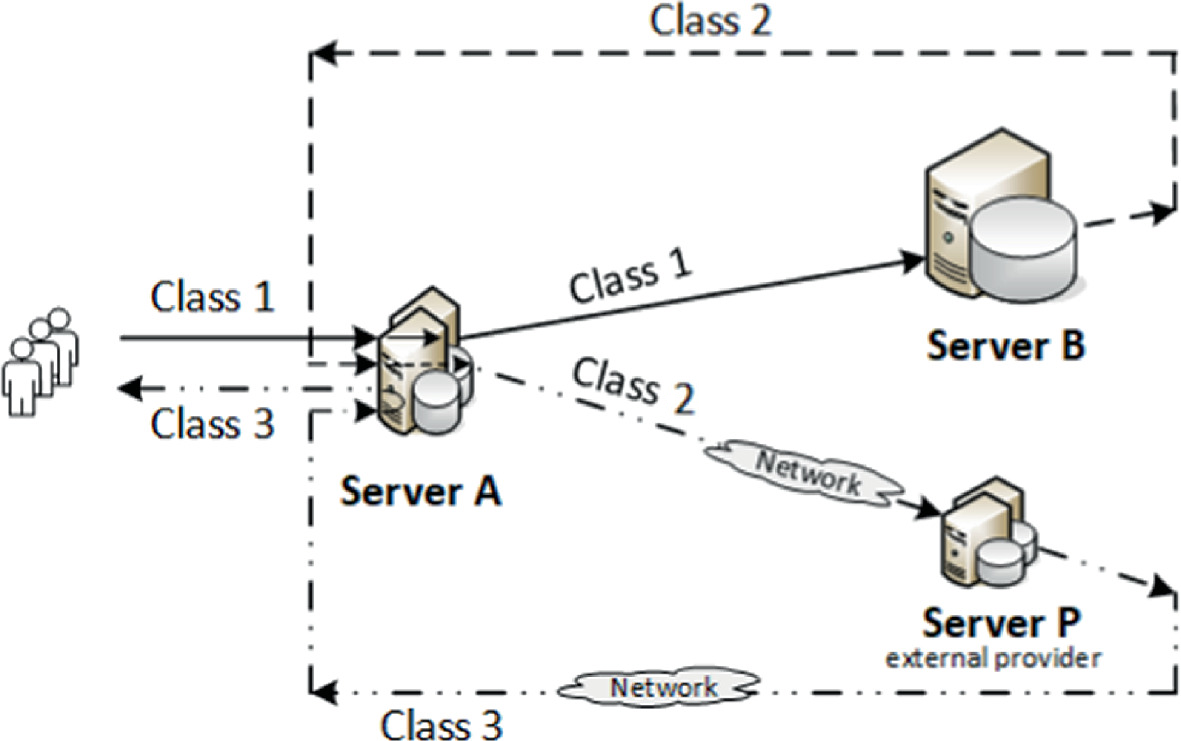
\includegraphics[width=0.8\linewidth]{figs/job_classes.png}
        \caption{Vista Bird-Eye dell'architettura distribuita della Web App. \citep{DBLP:books/sp/Serazzi24}}
        \label{fig:enter-label}
    \end{figure}
\end{frame}
